%%%%%%%%%%%%%%%%%%%%%%%%%%%%%%%%%%%%%%%%%%%%%%%%%%%%%%%%%%%%%%%%%%%%%%%%%%%%%%%%%%%%%%%%%%%%%%%%%%%%%%%%%%%%%%%%%%%%%%%%%%%%%%%%%%%%%%%%%%%%%%%%%%%%%%%%%%%%%%%%%%%%%%%%%%%%%%%%%%%%%%%%%%%%
% Written By Michael Brodskiy
% Class: AP Chemistry
% Professor: J. Morgan
%%%%%%%%%%%%%%%%%%%%%%%%%%%%%%%%%%%%%%%%%%%%%%%%%%%%%%%%%%%%%%%%%%%%%%%%%%%%%%%%%%%%%%%%%%%%%%%%%%%%%%%%%%%%%%%%%%%%%%%%%%%%%%%%%%%%%%%%%%%%%%%%%%%%%%%%%%%%%%%%%%%%%%%%%%%%%%%%%%%%%%%%%%%%

\documentclass[12pt]{article} 
\usepackage{alphalph}
\usepackage[utf8]{inputenc}
\usepackage[russian,english]{babel}
\usepackage{titling}
\usepackage{amsmath}
\usepackage{graphicx}
\usepackage{enumitem}
\usepackage{amssymb}
\usepackage[super]{nth}
\usepackage{expl3}
\usepackage[version=4]{mhchem}
\usepackage{hpstatement}
\usepackage{rsphrase}
\usepackage{everysel}
\usepackage{ragged2e}
\usepackage{geometry}
\usepackage{fancyhdr}
\usepackage{cancel}
\usepackage{siunitx}
\usepackage{chemfig}
\geometry{top=1.0in,bottom=1.0in,left=1.0in,right=1.0in}
\newcommand{\subtitle}[1]{%
  \posttitle{%
    \par\end{center}
    \begin{center}\large#1\end{center}
    \vskip0.5em}%

}
\newcommand{\orbital}[2]{{%
    \def\+{\big|\hspace{-2pt}\overline{\underline{\hspace{2pt}\upharpoonleft}}}%
    \def\-{\overline{\underline{\downharpoonright\hspace{2pt}}}\hspace{-2pt}\big|}%
    \def\0{\big|\hspace{-2pt}\overline{\underline{\phantom{\hspace{2pt}\downharpoonright}}}}%
    \def\1{\overline{\underline{\phantom{\downharpoonright\hspace{2pt}}}}\hspace{-2pt}\big|}%
  \setlength\tabcolsep{0pt}% remove extra horizontal space from tabular
  \begin{tabular}{c}$#2$\\[2pt]#1\end{tabular}%
}}
\DeclareSIUnit\Molar{\textsc{m}}
\DeclareSIUnit\atm{\textsc{atm}}
\DeclareSIUnit\torr{\textsc{torr}}
\DeclareSIUnit\psi{\textsc{psi}}
\DeclareSIUnit\bar{\textsc{bar}}
\usepackage{hyperref}
\hypersetup{
colorlinks=true,
linkcolor=blue,
filecolor=magenta,      
urlcolor=blue,
citecolor=blue,
}

\urlstyle{same}


\title{Chapter 9 $-$ Liquids and Solids}
\date{\today}
\author{Michael Brodskiy\\ \small Instructor: Mr. Morgan}

% Mathematical Operations:

% Sum: $$\sum_{n=a}^{b} f(x) $$
% Integral: $$\int_{lower}^{upper} f(x) dx$$
% Limit: $$\lim_{x\to\infty} f(x)$$

\begin{document}

\maketitle

\begin{itemize}

  \item Evaporation $-$ When molecules escape the surface of a liquid

  \item What happens in a closed container:

    \begin{enumerate}

      \item Evaporation

      \item Condensation

    \end{enumerate}

  \item When the rate of evaporation equals the rate of condensation, equilibrium is reached.

  \item Vapor Pressure $-$ Pressure at equilibrium of a liquid, specific to a liquid, which is the max amount of molecules a vapor can hold. If there are not enough molecules, all are in vapor. If there are too many, liquid and vapor is mixed.

\item At High Vapor Pressure $-$ Weak forces, which means a lot of gas molecules, which means it is volatile (evaporates quickly)

\item At Low Vapor Pressure $-$ Forces are strong, resulting in few gas molecules, which means it is nonvolatile (evaporates slowly)

\item As temperature goes up, vapor pressure goes up

\item Boiling Point $-$ A liquid boils when it reaches the temperature at which the vapor pressure is equal to the pressure above it

\item Decreasing external pressure causes decrease in boiling point (don't cook pasta at Tahoe)

\item Critical Temperature $-$ A temperature above which the liquid phase can not exist

\item Critical Pressure $-$ The pressure that must be applied to cause condensation at the critical temperature

\item A phase diagram looks as follows:

  \begin{figure}[H]
    \centering
    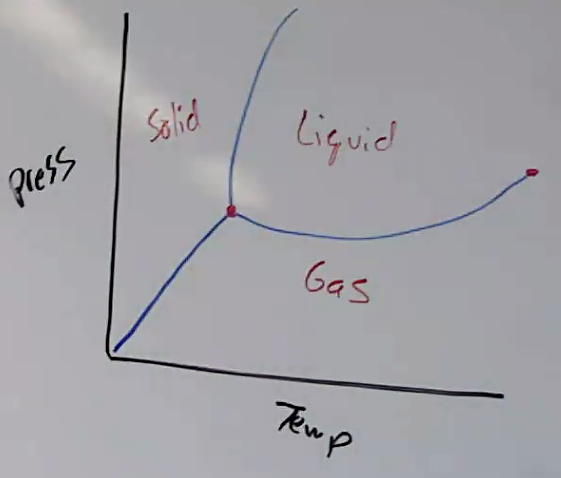
\includegraphics{Figures/PhaseDiagram.png}
    \caption{Phase Diagram Example}
    \label{fig:1}
  \end{figure}

\item On the line between gas and solid is sublimation

\item Point in the middle is the triple point

\item Between gas and liquid is boiling point line

\item Melting/Freezing line is between solid and liquid

\item Intramolecular forces (bonds)

  \begin{enumerate}

    \item Covalent

    \item Polar Covalent

    \item Ionic

  \end{enumerate}

\item Intermolecular Forces (Hold Molecules together)

  \begin{enumerate}

    \item Hydrogen Bonding $-$ \ce{H} with an \ce{N}, \ce{O}, \ce{F}: Strongest, highest melting and boiling points, but low vapor pressure.

    \item Dipole $-$ Between polar molecules.
      
      \item Dispersion (London) $-$ Between nonpolar molecules. Weakest of the three.

  \end{enumerate}

  \textit{Example: Which has the weakest force, lowest melting, and highest vapor pressure?}

\item \ce{C2H3OH} or \underline{\ce{C2H6}}

\item \ce{CH3CH2CH2OH} or \underline{\ce{CH3OH}}
  
\item \ce{H2O} or \underline{\ce{CH3OH}}
  
\item \underline{\ce{Ar54}} or \ce{NH3}

\item \underline{\ce{F2}} or \ce{Br2}

\item \ce{NO} or \underline{\ce{O2}}

  \textit{For the AP Exam:}

\item If a molecule uses hydrogen bonding, it uses dipole and dispersion. If it uses Dipole, it uses dipole and london. If it uses london, it uses only london.

\item Types of solids:

  \begin{enumerate}

    \item Molecular $-$ Uses one of the three intermolecular forces, low melting point, and non-conductive.

    \item Ionic $-$ Made of ions, high melting point, conducts if dissolved in water.

    \item Network Covalent $-$ Use intramolecular forces, very high melting point, nonconductive (\ce{C}, \ce{Si}, \ce{SiO}).

    \item Metals $-$ Use the electron sea diagram. Positive ions are held together in a mobile sea of electrons, and are very conductive.

  \end{enumerate}

\item The lattice energy is a measure of the strength of the ionic bond. The smaller the ions, the closer they approach one another, the stronger the bond is.

  \textit{Example: Which has the highest boiling point?}

\item \underline{\ce{Ca(OH)2}} or \ce{CH3OH}

\item \ce{NaCl} or \underline{\ce{SiO2}}

\item \underline{\ce{MgCl2}} or \ce{Cl2}

\end{itemize}


\end{document}

